\documentclass[xcolor=table,aspectratio=169]{beamer}
%!TEX root = thesis.tex

% Set german to default language and load english as well
\usepackage[english,ngerman]{babel}

% Set UTF8 as input encoding
\usepackage[utf8]{inputenc}

% Set T1 as font encoding
\usepackage[T1]{fontenc}
% Load a slightly more modern font
\usepackage{lmodern}
% Use the symbol collection textcomp, which is needed by listings.
\usepackage{textcomp}
% Load a better font for monospace.
\usepackage{courier}
% Load package to configure header and footer
\usepackage{scrlayer-scrpage}

% Set some options regarding the document layout. See KOMA guide
\KOMAoptions{%
  paper=a4,
  fontsize=12pt,
  parskip=half,
  headings=normal,
  BCOR=1cm,
  headsepline=0.5pt,
  DIV=12}

% do not align bottom of pages
\raggedbottom

% set style of captions
\setcapindent{0pt} % do not indent second line of captions
\setkomafont{caption}{\small}
\setkomafont{captionlabel}{\bfseries}
\setcapwidth[c]{0.9\textwidth}

% set the style of the bibliography
\bibliographystyle{alphadin}

% load extended tabulars used in the list of abbreviation
\usepackage{tabularx}

% load the color package and enable colored tables
\usepackage[table]{xcolor}

% define new environment for zebra tables
\newcommand{\mainrowcolors}{\rowcolors{1}{maincolor!25}{maincolor!5}}
\newenvironment{zebratabular}{\mainrowcolors\begin{tabular}}{\end{tabular}}
\newcommand{\setrownumber}[1]{\global\rownum#1\relax}
\newcommand{\headerrow}{\rowcolor{maincolor!50}\setrownumber1}

% add main color to section headers
\addtokomafont{chapter}{\color{maincolor}}
\addtokomafont{section}{\color{maincolor}}
\addtokomafont{subsection}{\color{maincolor}}
\addtokomafont{subsubsection}{\color{maincolor}}
\addtokomafont{paragraph}{\color{maincolor}}

% do not print numbers next to each formula
\usepackage{mathtools}
\mathtoolsset{showonlyrefs}
% left align formulas
\makeatletter
\@fleqntrue\let\mathindent\@mathmargin \@mathmargin=\leftmargini
\makeatother

% Allow page breaks in align environments
\allowdisplaybreaks

% header and footer
\pagestyle{scrheadings}
\setkomafont{pagenumber}{\normalfont\sffamily\color{maincolor}}
\setkomafont{pageheadfoot}{\normalfont\sffamily}
\setkomafont{headsepline}{\color{maincolor}}

% German guillemets quotes
\usepackage[german=guillemets]{csquotes}

% load TikZ to draw diagrams
\usepackage{tikz}

% load additional libraries for TikZ
\usetikzlibrary{%
  automata,%
  positioning,%
}

% set some default options for TikZ -- in this case for automata
\tikzset{
  every state/.style={
    draw=maincolor,
    thick,
    fill=maincolor!18,
    minimum size=0pt
  }
}

% load listings package to typeset sourcecode
\usepackage{listings}

% set some options for the listings package
\lstset{%
  upquote=true,%
  showstringspaces=false,%
  basicstyle=\ttfamily,%
  keywordstyle=\color{keywordcolor}\slshape,%
  commentstyle=\color{commentcolor}\itshape,%
  stringstyle=\color{stringcolor}}

% enable german umlauts in listings
\lstset{
  literate={ö}{{\"o}}1
           {Ö}{{\"O}}1
           {ä}{{\"a}}1
           {Ä}{{\"A}}1
           {ü}{{\"u}}1
           {Ü}{{\"U}}1
           {ß}{{\ss}}1
}

% define style for pseudo code
\lstdefinestyle{pseudo}{language={},%
  basicstyle=\normalfont,%
  morecomment=[l]{//},%
  morekeywords={for,to,while,do,if,then,else},%
  mathescape=true,%
  columns=fullflexible}

% load the AMS math library to typeset formulas
\usepackage{amsmath}
\usepackage{amsthm}
\usepackage{thmtools}
\usepackage{amssymb}

% load the paralist library to use compactitem and compactenum environment
\usepackage{paralist}

% load varioref and hyperref to create nicer references using vref
\usepackage[ngerman]{varioref}
\PassOptionsToPackage{hyphens}{url} % allow line break at hyphens in URLs
\usepackage{hyperref}

% setup hyperref
\hypersetup{breaklinks=true,
            pdfborder={0 0 0},
            ngerman,
            pdfhighlight={/N},
            pdfdisplaydoctitle=true}

% Fix bugs in some package, e.g. listings and hyperref
\usepackage{scrhack}

% define german names for referenced elements
% (vref automatically inserts these names in front of the references)
\labelformat{figure}{Abbildung\ #1}
\labelformat{table}{Tabelle\ #1}
\labelformat{appendix}{Anhang\ #1}
\labelformat{chapter}{Kapitel\ #1}
\labelformat{section}{Abschnitt\ #1}
\labelformat{subsection}{Unterabschnitt\ #1}
\labelformat{subsubsection}{Unterunterabschnitt\ #1}

% define theorem environments
\declaretheorem[numberwithin=chapter,style=plain]{Theorem}
\labelformat{Theorem}{Theorem\ #1}

\declaretheorem[sibling=Theorem,style=plain]{Lemma}
\labelformat{Lemma}{Lemma\ #1}

\declaretheorem[sibling=Theorem,style=plain]{Korollar}
\labelformat{Korollar}{Korollar\ #1}

\declaretheorem[sibling=Theorem,style=definition]{Definition}
\labelformat{Definition}{Definition\ #1}

\declaretheorem[sibling=Theorem,style=definition]{Beispiel}
\labelformat{Beispiel}{Beispiel\ #1}

\declaretheorem[sibling=Theorem,style=definition]{Bemerkung}
\labelformat{Bemerkung}{Bemerkung\ #1}

%!TEX root = thesis.tex

% Use this file to define some macros you need in your thesis. A macro is a short command that inserts some mathematical symbols or texts you do not want to retype each time you need some. I recommend to use as many macros as possible, because you are able to change them later. For example if you use the same macro each time you need to give the formal semantics of an expression you can easily change the appearance of these brackets by updating the macro later on.

% Set of natural numbers
\newcommand{\N}{\mathbb{N}}

% The default epsilon does not look very nice
\let\epsilon\varepsilon

% If you need to use mathematical expressins like an epsilon in the section titles of your thesis you will end up with warnings that these special symbols cannot be included in the PDF favorites. The following macro uses the mathematical symbol during the text of the thesis and the string "Epsilon" in the PDF favorites.
\newcommand{\pdfepsilon}{\texorpdfstring{$\epsilon$}{Epsilon}}


\author{Julian Huber}
\title{LaTeX}
\date{MCI 2022}

\begin{document}

%!TEX root = latex.tex

\begin{frame}
  \begin{center}
    \vskip1cm
    {\bfseries\color{maincolor}{\fontsize{72pt}{72pt}\selectfont\rmfamily\LaTeX}
    \par\vskip5mm
    \Huge Introduction}
    \par\vskip12mm
    \large Dr. Julian Huber - Translated from Malte Schmitz \footnote{\url{https://github.com/malteschmitz/latex-talk}}
  \end{center}
\end{frame}
%!TEX root = latex.tex

\begin{frame}{Learning Goals}
  \begin{itemize}
    \item get to know \LaTeX\
    \item structure von \LaTeX-documents, -commands and -environments.
    \item application of \LaTeX\ for papers and theses.
    \item where to use and not to use \LaTeX.
  \end{itemize}
\end{frame}

\begin{frame}{Table of Content}
  \tableofcontents
\end{frame}

\begin{frame}{Website}
  \vskip-4ex\hfill\parbox{6cm}{\centering
    
\includegraphics[width=6cm]{qrcode}\\[1ex]
    \href{http://www.mlte.de/latex}{\huge\texttt{mlte.de/latex}}}
  \begin{itemize}
    \item German original of this presentation.
    \item script for this presentation.
    \item links to \LaTeX\ distributions, IDEs and further reading.
  \end{itemize}
\end{frame}


\section{What is \LaTeX?}
%!TEX root = latex.tex

\subsection{Context}

\begin{frame}{Dimensions of a Document}
  \begin{onlyenv}<presentation:1| article:0>
    \begin{center}
      Content is the meaning of a document.
    \end{center}
  \end{onlyenv}
  \begin{onlyenv}<presentation:2| article:0>
    \begin{description}
      \item[\textnormal{\color{black}Content}] is the \emph{meaning} of a document.
      \item[\textnormal{\color{black}Structure}] is the \emph{outline }  of a document.
      \uncover<3>{\item Foo}
    \end{description}
  \end{onlyenv}
  \begin{onlyenv}<3>
    \begin{description}
      \item[Content] is the \alert{meaning}  of a document.
      \item[Structure] is the \alert{outline}  of a document.
      \item[Form] is the \alert{apperance} of a document.
    \end{description}
  \end{onlyenv}
\end{frame}

\begin{frame}{Structure vs. Form}
  \begin{Beispiele}[Structure]
    \begin{itemize}
      \item heading
      \item grouping
      \item listing
    \end{itemize}
  \end{Beispiele}

  \xxx

  \begin{Beispiele}[Form]
    \begin{itemize}
      \item 13{,}37~cm wide coloured box
      \item 0{,}6~cm indentation
      \item bullet $\blacktriangleright$ at beginning of the column
    \end{itemize}
  \end{Beispiele}
\end{frame}

\begin{frame}[fragile]{Markdown Languages}
  \newcommand{\entry}[2]{\draw[maincolor, thick] (-.2,#1) -- (.2,#1) node[right] {\color{black}#2};}
  \hskip 8ex\begin{tikzpicture}
    \draw[maincolor, thick] (0,0) node[below] {\textbf{Form}} edge[<->] (0,6);
    \draw[maincolor] (0,6) node[above] {\textbf{Struktur}};
    \entry{.5}{Pixel graphics e.\,g. Paint};
    \entry{1}{Vector graphics e.\,g. Inkscape};
    \entry{1.5}{PDF};
    \entry{2.5}{\TeX};
    \entry{3}{DTP-Tools  e.\,g. Scribus};
    \entry{3.5}{Office Word, Writer, \ldots};
    \entry{4}{\textcolor{examplecolor}{\LaTeX}};
    \entry{4.75}{HTML};
    \entry{5.5}{Outliner};
  \end{tikzpicture}
\end{frame}

\begin{frame}{\LaTeX\ vs. Office Word}
  \begin{center}
    \begin{tikzpicture}[thick]
      \draw[->] (0,0) -- node[below] {Document size and -complexity} (8,0);
      \draw[->] (0,0) -- node[rotate=90, above] {Effort and time requirement} (0,6);
      \begin{scope}[
          every node/.style={font=\Large},
        ]
        \draw[alertedcolor, domain=0:3.68965] plot (\x, {exp(\x+.5)/12 + .5});
        \path[alertedcolor, domain=0:3.3] plot (\x, {exp(\x+.5)/12 + .5}) node[above left] {Office Word};
        \pause
        \draw[dashed, maincolor] (0,5.5) -- node[above,near end] {hopeless} (8,5.5);
        \pause
        \draw[examplecolor, domain=0:8] plot (\x, {\x^2/25 + 1.5});
        \path[examplecolor, domain=0:6] plot (\x, {\x^2/25 + 1.5}) node[below right] {\LaTeX};
      \end{scope}
    \end{tikzpicture}
  \end{center}
\end{frame}

\subsection{\LaTeX-Documents}

\begin{frame}[fragile]{A \LaTeX-Document}
  \begin{itemize}
    \item<1-> are pure \alert{text files} with \alert{content}
    \item<2-> also contain \alert{structure} of the content
    \item<3-> typesetting is done by \LaTeX\  \alert{separately}
  \end{itemize}

  \xxx
  
  \begin{center}
    \begin{tikzpicture}[
        shorten <=5pt,
        shorten >=5pt
      ]
      \matrix[column sep=3em] {
        \node[text width=6em] (source) {
          \only<1>{\lstinputlisting[
              basicstyle=\ttfamily\fontsize{4}{4}\selectfont 
            ]{demo/exampleContent.txt}}
          \only<2->{\lstinputlisting[
              basicstyle=\ttfamily\fontsize{4}{4}\selectfont,
              linerange={1-1,12-27}
            ]{demo/example.tex}}
        };
        &
        \visible<3->{\node[inner sep=0pt] (latex)
          {\rmfamily\Large\bfseries\LaTeX};}
        &
        \visible<3->{\node[draw=maincolor, thick] (pdf) {
          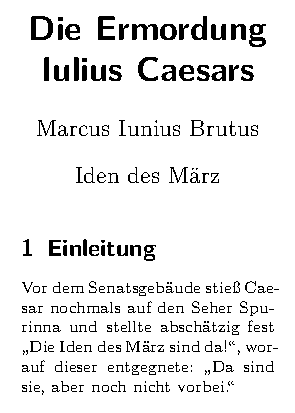
\includegraphics[width=6em]{demo/example.pdf}
        };}\\
        \node {\shortstack{Content \visible<2->{\&\\ Structure}}};
        & & 
        \visible<3->{\node {\shortstack{typeset\\Document}};}\\
      };
      \visible<3->{\path[very thick, ->]
        (source) edge (latex)
        (latex) edge (pdf);}
    \end{tikzpicture}
  \end{center}
\end{frame}


\section{Installing \LaTeX}
%!TEX root = latex.tex

\subsection{Toolbox}

	
\begin{frame}[fragile]{What You need to start}
	\begin{itemize}
		\item<1-> \alert{Distribution} that compiles the text
		\item<2-> user friendly \alert{Editor} to edit the \LaTeX-Document
		\item<3-> \alert{Literature tool} if You want to manage many citations
	\end{itemize}
	
	\xxx
	
	\begin{center}
		\begin{tikzpicture}[
			shorten <=5pt,
			shorten >=5pt
			]
			\matrix[column sep=3em] 
				{
					\visible<1->{\node[] {
							
\includegraphics[width=6em]{demo/MikTex.png}
						};} &
						\visible<2->{\node[] {
							
\includegraphics[width=6em]{demo/1024px-TeXstudio_Logo.svg.png}
						};} &
						 	\visible<3->{\node[] {
						 		
\includegraphics[width=6em]{demo/JabRef-icon-256.png}
					 		};} \\
					\visible<1->{\node {\shortstack{e.g., TexLive\\MikTex}};}  &\visible<2->{\node {\shortstack{e.g., TexStudio\\Texmaker}};}  &  \visible<3->{\node {\shortstack{e.g., JabRef\\Citavi}};} \\
				};

		\end{tikzpicture}
	\end{center}

\end{frame}
\livecoding{What is \LaTeX{}}


\section{Using \LaTeX{}}
\subsection{Markups, Commands and Environments}
\livecoding{Using \LaTeX{}}


\section{Structure and Preamble}
%!TEX root = latex.tex

\subsection{Structure of a Document}

\begin{frame}[fragile]{Structure of a Document}
  \begin{tikzpicture}[%
      auto,
      every edge/.style={
        draw,
        decorate,
        decoration=brace,
        very thick
      }
    ]
    \node[text width=\textwidth, anchor=south] (tex) {
      \begin{lstlisting}[gobble=8]
        \documentclass{scrartcl}

        \usepackage[ngerman]{babel}
        \usepackage[utf8]{inputenc}
        \usepackage[T1]{fontenc}

        \KOMAoptions{%
          parskip=full,%
          fontsize=12pt}

        \begin{document}
          Franz jagt im komplett
          verwahrlosten Taxi quer
          durch Bayern.
        \end{document}
      \end{lstlisting}
    };

    \pause
    \draw
      (1,7.6) edge node {Dokument class} (1,7.2);
    \pause
    \draw
      (1,6.6) edge node {\shortstack{loading\\packages}} (1,5.3);
    \pause
    \draw
      (0,4.7) edge node {Settings} (0,3.5);
    \pause
    \draw
      (3,6.6) edge node {Preamble} (3,3.5);
    \pause
    \draw
      (1,2.6) edge node {Document body} (1,.9);
  \end{tikzpicture}
\end{frame}

\subsection{Dokument classes}

\begin{frame}[fragile]{Dokument classes}
		\lstinline-\documentclass{scrartcl}-\newline
short articles

\xxx

\lstinline-\documentclass{scrreprt}-\newline
Reports with  covering page and chapters

\xxx

\lstinline-\documentclass{scrbook}-\newline
double-pages book with parts, chapters and headers 
		
		
\end{frame}



\subsection{Loading packages}

\begin{frame}[fragile]{Praeamble: Standard packages}
  \lstset{
    backgroundcolor={},
    frame=no,
    gobble=4,
    aboveskip=3ex,
    belowskip=0pt
  }
  
  \begin{lstlisting}
    \usepackage[utf8]{inputenc}
  \end{lstlisting}
  UTF-8 for text encoding
  
  \begin{lstlisting}
    \usepackage[ngerman]{babel}
  \end{lstlisting}
  German hyphenation, date formats etc.
  
  \begin{lstlisting}
    \usepackage[T1]{fontenc}
  \end{lstlisting}
  improves text encoding for western european languages
  
  \begin{lstlisting}
    \usepackage{lmodern}
  \end{lstlisting}
  more modern fonts
\end{frame}

\begin{frame}[fragile]{Präambel: zusätzliche Pakete}
  \lstset{
    backgroundcolor={},
    frame=no,
    gobble=4,
    aboveskip=3ex,
    belowskip=0pt
  }

  \begin{lstlisting}
    \usepackage{xcolor}
  \end{lstlisting}
  adds command \lstinline-\textcolor- fo colour

  \begin{lstlisting}
    \usepackage{graphicx}  
  \end{lstlisting}
  adds command \lstinline-\includegraphics- for figures

  \begin{lstlisting}
    \usepackage[german=guillemets]{csquotes}
  \end{lstlisting}
  adds command \lstinline-\enquote- for parentheses

  \begin{lstlisting}
    \usepackage{amsmath}
  \end{lstlisting}
  adds environment \lstinline-align- for aligned mathematical formulas

  \begin{lstlisting}
    \usepackage[breaklinks=true]{hyperref}
  \end{lstlisting}
  improves pdf creation (e.g. hyperlinks)
\end{frame}

\livecoding{Structure of a Document}

\section{Theses}
%!TEX root = latex.tex

\begin{frame}{Theses}
  \centerline{\begin{tikzpicture}
      \node[fill=white,blur shadow,inner sep=0pt,draw=gray,very thin] {
        \pgfimage[height=8cm]{demo/thesis-titlepage}
      };
    \end{tikzpicture}}
\end{frame}

\subsection{Modular Documents, and Sections}
%!TEX root = latex.tex

\begin{frame}{Modular Documents}
  \tikzset{
    every node/.style={
      inner sep=1pt,
      on grid,
      label position=below,
      auto
    },
    shorten >=1em,
    shorten <=1em,
    node distance=7em and 5em
  }
  \begin{center}
    \begin{tikzpicture}
      \node[inner sep=10pt] (large) {\tikz\node[examplecolor,label=\texttt{\ \ main}] {\only<presentation:1| article:0>{\icon[2]{TEX}}\only<presentation:2| article:0>{\icon[10]{TEX}}\only<presentation:3| article:0>{\icon[20]{TEX}}\only<4->{\icon[30]{TEX}}};};
      \onslide<5->
      \path[alertedcolor, line width=3pt, line cap=round, shorten >=0pt,shorten <=0pt]
        (large.north east) edge (large.south west)
        (large.north west) edge (large.south east);
    \end{tikzpicture}
    \qquad
    \only<6->{%
      \begin{tikzpicture}
        \node[examplecolor,label=below:\texttt{\ \ main}] (main) {\icon[1]{TEX}};

        \uncover<7->{%
          \node[maincolor,label=\texttt{\ \ styles}, above left=of main] (config) {\icon[2]{TEX}};
          \path[very thick]
            (config.east) edge[->] node[pos=.6, swap]
              {\texttt{\color{texcs}\bfseries\textbackslash input}} (main);
        }

        \uncover<8->{%
          \node[maincolor,label=\texttt{\ \ intro}, above right=of main] (chap1) {\icon[3]{TEX}};
          \path[very thick]
            (chap1.west) edge[->] node[pos=.6]
              {\texttt{\color{texcs}\bfseries\textbackslash include}} (main);
        }

        \uncover<9->{%
          \node[maincolor,label=\texttt{\ \ methods}, below right=of main] (chap2) {\icon[5]{TEX}};
          \path[very thick]
            (chap2.west) edge[->,shorten >=1.6em] node[pos=.5, swap]
              {\texttt{\color{texcs}\bfseries\textbackslash include}} (main);
        }

        \uncover<10->{%
          \node[maincolor,label=\texttt{\ \ summary}, below left=of main] (chap3) {\icon[4]{TEX}};
          \path[very thick]
            (chap3.east) edge[->,shorten >=1.6em] node[pos=.5]
              {\texttt{\color{texcs}\bfseries\textbackslash include}} (main);
        }
      \end{tikzpicture}
    }
  \end{center}
\end{frame}

\begin{frame}[fragile]{Modular Structure}
  \begin{columns}
    \column{.4\textwidth}
    \begin{tikzpicture}[
        node distance=0,
        grow via three points={one child at (0,-0.7) and two children at (0,-0.7) and (0,-1.4)},
        edge from parent path={([xshift=6pt]\tikzparentnode.south west) |- (\tikzchildnode.west)},
        every node/.style={thick,anchor=west,xshift=-3mm,font=\ttfamily,text width=4em},
        every child/.style={thick,draw=black},
        dir/.style={draw=maincolor,fill=maincolor!10},
        optional/.style={dashed}
      ]
      \node [dir] {thesis}
        child { node [dir] {inc}
          child { node {title}}
          child { node {styles}}
        }
        child [missing] {}
        child [missing] {}
        child { node [dir] {content}
          child { node {intro}}
          child { node (methods) {methods}}
          child { node (summary) {summary}}
        }
        child [missing] {}
        child [missing] {}
        child [missing] {}
        child { node {main}};
        \only<2>\path[alertedcolor, line width=1pt, line cap=rounded]
          (methods.south west) edge (methods.north east);
        \only<2>\path[alertedcolor, line width=1pt, line cap=rounded]
          (summary.south west) edge (summary.north east);
      \end{tikzpicture}
    \column{0.6\textwidth}
    \begin{lstlisting}[gobble=6,escapechar=-]
      \documentclass{scrbook}
      \input{inc/styles}
      -\alt<2>{\textcolor{texcs}{\bfseries\textbackslash includeonly}\textcolor{red}{\bfseries\{}content/intro\textcolor{red}{\bfseries\}}}{\textcolor{comment}{\itshape\% \textbackslash includeonly}}-
      \begin{document}
        \frontmatter
        %!TEX root = thesis.tex

\begin{titlepage}
  \thispagestyle{empty}

  \vskip1cm

  \pgfimage[height=2.5cm]{uni-logo-example\imagesuffix}
  
  \vskip2.5cm
  
  \LARGE
  
  \textbf{\sffamily\color{maincolor}Über Gummibärchen}

  \textit{On Gummy Bears}

  \normalfont\normalsize

  \vskip2em
  
  \textbf{\sffamily\color{maincolor}Masterarbeit}

  im Rahmen des Studiengangs \\
  \textbf{\sffamily\color{maincolor}Informatik} \\
  der Universität zum Beispiel

  \vskip1em

  vorgelegt von \\
  \textbf{\sffamily\color{maincolor}Max Mustermann}

  \vskip1em
  
  ausgegeben und betreut von \\
  \textbf{\sffamily\color{maincolor}Prof. Dr. Erika Musterfrau}

  \vskip1em

  mit Unterstützung von\\
  Lieschen Müller

  \vskip1em

  Die Arbeit ist im Rahmen einer Tätigkeit bei der Firma Muster GmbH entstanden.


  \vfill

  Musterhausen, den \duedate
\end{titlepage}

        \tableofcontents

        \mainmatter
        \include{content/intro}
        \include{content/methods}
        %!TEX root = basic.tex

\begin{frame}[label=basics-summary]{Zusammenfassung}
  \begin{enumerate}
    \item Das \alert{\LaTeX-Dokument} enthält \alert{Inhalt und Struktur}.
    \item \LaTeX\ setzt ein druckfertiges \alert{PDF-Dokument} und kümmert sich dabei um die \alert{gute Form}.
    \item Es ist schwierig, \alert{neue Layouts} zu erzeugen.
    \item Ein \LaTeX-Dokument besteht aus \alert{Dokumentenklasse}, \alert{Präambel} und \alert{Dokumentenkörper}.
    \item Wir haben \alert{Auszeichnungen}, \alert{Formelsatz}, \alert{Listen}, \alert{Tabellen}, \alert{Abbildungen}, \alert{Verzeichnisse} und \alert{Verweise} kennen gelernt.
  \end{enumerate}
\end{frame}

\begin{frame}[fragile]{Zum Weiterlesen}
  \begin{mybib}
    \bibitem{Wiki}
      Wikibooks contributors.
      \newblock \emph{\LaTeX\ Wikibook},
      \newblock \alt<presentation>{\href{http://en.wikibooks.org/wiki/LaTeX}{\texttt{en.wikibooks.org/LaTeX}}}{\url{http://en.wikibooks.org/wiki/LaTeX}}, November 2014
    \bibitem{basics_Kohm}
      Markus Kohm, Jens-Uwe-Morawski.
      \newblock \emph{KOMA-Script},
      \newblock \alt<presentation>{\href{http://mirrors.ctan.org/macros/latex/contrib/koma-script/doc/scrguide.pdf}{\texttt{scrguide.pdf}}}{\url{http://mirrors.ctan.org/macros/latex/contrib/koma-script/doc/scrguide.pdf}}, Dezember 2013.
  \end{mybib}
\end{frame}

\begin{frame}[fragile]{Zum weiteren Weiterlesen}
  \begin{mybib}
    \bibitem{basics_Kopka}
      Helmut Kopka.
      \newblock \emph{\LaTeX, Band 1: Einführung},
      \newblock Addison-Wesley, März 2002.
    \bibitem{basics_Braune}
      Klaus Braune, Joachim und Marion Lammarsch.
      \newblock \emph{\LaTeX: Basissystem, Layout, Formelsatz},
      \newblock Addison-Wesley, Mai 2006.
    \bibitem{Struckmann}
      Werner Struckmann.
      \newblock \emph{Einige typographische Grundregeln und ihre Umsetzung in \LaTeX},
      \newblock \alt<presentation>{\href{http://www2.informatik.hu-berlin.de/sv/lehre/typographie.pdf}{\texttt{typographie.pdf}}}{\url{http://www2.informatik.hu-berlin.de/sv/lehre/typographie.pdf}}, September 2007.
  \end{mybib}
\end{frame}


      \end{document}
    \end{lstlisting}
  \end{columns}
\end{frame}

\begin{frame}[fragile]{Commands for a modular Structure}
  \begin{tabular}{rL{6cm}}
    \lstinline-\input- & add content of the file. \\[1ex]
    \lstinline-\include- & add content of the file and \newline
      add pagebreaks before and behind.\\[1ex]
    \lstinline-\includeonly- & list of files regarded \newline by \lstinline-\include- 
      .\\
  \end{tabular}
\end{frame}

\begin{frame}[fragile]{Segments of long Documents (\lstinline-scrbook-)}
  \begin{lstlisting}[gobble=4]
    \begin{document}
      \frontmatter % Titlepage, Table of Content, etc.
      \begin{titlepage} ... \end{titlepage}
      \tableofcontents
	  	% Has Roman page numbering (i, ii, ...)
      \mainmatter % Main content
      \chapter{Einleitung}
		% Has Arabic page numbering (1, 2, ...)
      \appendix % Appendix, Bibliography
      \chapter{Glossar}
      
      \backmatter % Ending
      \listoffigures
    \end{document}
  \end{lstlisting}
\end{frame}

\begin{frame}[fragile]{Layout of the Segments}
  \begin{tabbing}
    \hskip8cm \= \kill

    \textcolor{texcs}{\ttfamily\bfseries\textbackslash frontmatter} Prefix
        \> \textcolor{examplecolor}{\bfseries\sffamily Abstract}\\
      \strut\ \textcolor{maincolor}{--} chapters not numbered \\
      \strut\ \textcolor{maincolor}{--} Roman page numbers
        \> \textcolor{examplecolor}{\rmfamily \qquad -- iv --} \\[3ex]

    \pause

    \textcolor{texcs}{\ttfamily\bfseries\textbackslash mainmatter} Main Content
        \> \textcolor{examplecolor}{\bfseries\sffamily 3. Konzept}\\
      \strut\ \textcolor{maincolor}{--} chapters numbered in Arabic\\
      \strut\ \textcolor{maincolor}{--} \alert{new} Arabic page numbers
        \> \textcolor{examplecolor}{\rmfamily \qquad -- 5 --} \\[3ex]

    \pause

    \textcolor{texcs}{\ttfamily\bfseries\textbackslash appendix} Appendix
        \> \textcolor{examplecolor}{\bfseries\sffamily A. Anhang}\\
      \strut\ \textcolor{maincolor}{--} \alert{new} alphabetic chapter numbers\\
      \strut\ \textcolor{maincolor}{--} Arabic page numbers
        \> \textcolor{examplecolor}{\rmfamily \qquad -- 126 --} \\[3ex]

    \pause

    \textcolor{texcs}{\ttfamily\bfseries\textbackslash backmatter} Postamble
        \> \textcolor{examplecolor}{\bfseries\sffamily Literatur}\\
      \strut\ \textcolor{maincolor}{--} chapters not numbered \\
      \strut\ \textcolor{maincolor}{--} Arabic page numbers
        \> \textcolor{examplecolor}{\rmfamily \qquad -- 135 --}
  \end{tabbing}
\end{frame}


\subsection{Sections, Math, Lists, Tables and Figures}
\livecoding{Special Environments \LaTeX}


%\subsection{Theorems}
%\livecoding{Theorems}

\subsection{Bibliographies with \texorpdfstring{\BibTeX}{BibTeX}}
%!TEX root = advanced.tex

\begin{frame}{Bibliographies with \texorpdfstring{\BibTeX}{BibTeX}}
  \centerline{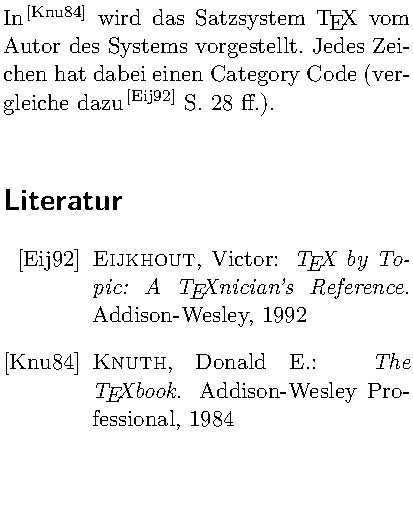
\includegraphics[width=9cm]{demo/arbeit.pdf}}
\end{frame}

\begin{frame}[fragile]{Das \LaTeX-Dokument \texttt{arbeit.tex}}
  \begin{lstlisting}[gobble=4]
    \documentclass{scrartcl}
    %...
\usepackage [super , square , sort&compress ]{natbib}

	\begin{document}
		In \cite{Knuth} wird das Satzsystem 
		\TeX{} vom Autor des Systems
		vorgestellt. Jedes Zeichen hat dabei
		einen Category Code (vergleiche dazu
		\cite[S.~28~ff.]{Eijkhout}).
		
		\bibliographystyle{alphadin}
		
		\bibliography{datenbank}
	\end{document}
  \end{lstlisting}
\end{frame}

\begin{frame}{The literature data base \texttt{datenbank.bib}}
  \lstinputlisting[language=BibTeX,moretexcs={TeX}]{demo/datenbank.bib}
\end{frame}

\begin{frame}[fragile]{Compilation}
  \begin{lstlisting}[language={},morekeywords={pdflatex,bibtex},gobble=4]
    pdflatex arbeit
    bibtex arbeit
    pdflatex arbeit
    pdflatex arbeit
  \end{lstlisting}

  \xxx
  \pause

  \vskip -3.1cm
  \begin{tikzpicture}
    \draw[red,very thick] (0,0) -- (2.8cm, 2.7cm);
  \end{tikzpicture}
  \vskip .5cm

  \begin{lstlisting}[language={},morekeywords={latexmk},gobble=4]
    latexmk -pdf arbeit
  \end{lstlisting}
\end{frame}

\begin{frame}{How does \BibTeX work?}
  \begin{tikzpicture}[
      on grid,
      node distance=9mm and 23mm,
      engine/.style={
        font=\rmfamily\Large\bfseries,
        inner sep=2pt
      }
    ]

    \uncover<2->{\node[engine] (pdftex1) {\pdfTeX};}
    \uncover<1->{\node[left=40mm of pdftex1, texicon] (tex) {\icon{TEX}};}
    \uncover<1->{\node[right=40mm of pdftex1, bibicon] (bib) {\icon{BIB}};}
    \uncover<3->{\node[below left=18mm and 23mm of pdftex1, auxicon] (aux1) {\icon{AUX}};}
    \uncover<3>{\node[below right=of pdftex1, pdficon] (pdf1) {\icon{PDF}};}
    \uncover<4->{\node[below right=of pdftex1, pdficon!30] {\icon{PDF}};}
    \uncover<4->{\node[below=18mm of pdftex1, engine] (bibtex) {\BibTeX};}
    \uncover<5->{\node[below right=of bibtex, bblicon] (bbl) {\icon{BBL}};}
    \uncover<6->{\node[below=18mm of bibtex, engine] (pdftex2) {\pdfTeX};}
    \uncover<7->{\node[below left=of pdftex2, auxicon] (aux2) {\icon{AUX}};}
    \uncover<7>{\node[below right=of pdftex2, pdficon] (pdf2) {\icon{PDF}};}
    \uncover<8->{\node[below right=of pdftex2, pdficon!30] {\icon{PDF}};}
    \uncover<8->{\node[below=18mm of pdftex2, engine] (pdftex3) {\pdfTeX};}
    \uncover<9>{\node[below left=of pdftex3, auxicon] (aux3) {\icon{AUX}};}
    \uncover<10->{\node[below left=of pdftex3, auxicon!30] {\icon{AUX}};}
    \uncover<9->{\node[below right=of pdftex3, pdficon] (pdf3) {\icon{PDF}};}

    \uncover<2->{\path[very thick, ->]
      (tex) edge (pdftex1);}

    \uncover<3->{\path[very thick, ->]
      (pdftex1) edge (aux1)
                edge (pdf1);}

    \uncover<4->{\path[very thick, ->, black!30]
      (pdftex1) edge (pdf1);}

    \uncover<4->{\path[very thick, ->]
      (aux1) edge (bibtex);}

    \uncover<4->{\draw[very thick, ->]
      (bib.south) ++ (.2,0) |- (bibtex);}

    \uncover<5->{\path[very thick, ->]
      (bibtex) edge (bbl);}

    \uncover<6->{\draw[very thick, ->]
      (tex.south) ++ (.2,0) |- (pdftex2)
      (bbl.south) ++ (.2,0) |- (pdftex2);}

    \uncover<6->{\path[very thick, ->]
      (aux1) edge (pdftex2);}

    \uncover<7->{\path[very thick, ->]
      (pdftex2) edge (aux2)
                edge (pdf2);}

    \uncover<8->{\path[very thick, ->, black!30]
      (pdftex2) edge (pdf2);}

    \uncover<8->{\draw[very thick, ->]
      (tex.south) ++ (.2,0) |- (pdftex3)
      (bbl) -- (bib |- bbl) -- ++(.2,0) |- (pdftex3);}

    \uncover<8->{\path[very thick, ->]
      (aux2) edge (pdftex3);}

    \uncover<9->{\path[very thick, ->]
      (pdftex3) edge (aux3)
                edge (pdf3);}

    \uncover<10->{\path[very thick, ->, black!30]
      (pdftex3) edge (aux3);}
  \end{tikzpicture}
\end{frame}




\livecoding{Bibliographies in \LaTeX}

%!TEX root = basic.tex

\begin{frame}[label=basics-summary]{Zusammenfassung}
  \begin{enumerate}
    \item Das \alert{\LaTeX-Dokument} enthält \alert{Inhalt und Struktur}.
    \item \LaTeX\ setzt ein druckfertiges \alert{PDF-Dokument} und kümmert sich dabei um die \alert{gute Form}.
    \item Es ist schwierig, \alert{neue Layouts} zu erzeugen.
    \item Ein \LaTeX-Dokument besteht aus \alert{Dokumentenklasse}, \alert{Präambel} und \alert{Dokumentenkörper}.
    \item Wir haben \alert{Auszeichnungen}, \alert{Formelsatz}, \alert{Listen}, \alert{Tabellen}, \alert{Abbildungen}, \alert{Verzeichnisse} und \alert{Verweise} kennen gelernt.
  \end{enumerate}
\end{frame}

\begin{frame}[fragile]{Zum Weiterlesen}
  \begin{mybib}
    \bibitem{Wiki}
      Wikibooks contributors.
      \newblock \emph{\LaTeX\ Wikibook},
      \newblock \alt<presentation>{\href{http://en.wikibooks.org/wiki/LaTeX}{\texttt{en.wikibooks.org/LaTeX}}}{\url{http://en.wikibooks.org/wiki/LaTeX}}, November 2014
    \bibitem{basics_Kohm}
      Markus Kohm, Jens-Uwe-Morawski.
      \newblock \emph{KOMA-Script},
      \newblock \alt<presentation>{\href{http://mirrors.ctan.org/macros/latex/contrib/koma-script/doc/scrguide.pdf}{\texttt{scrguide.pdf}}}{\url{http://mirrors.ctan.org/macros/latex/contrib/koma-script/doc/scrguide.pdf}}, Dezember 2013.
  \end{mybib}
\end{frame}

\begin{frame}[fragile]{Zum weiteren Weiterlesen}
  \begin{mybib}
    \bibitem{basics_Kopka}
      Helmut Kopka.
      \newblock \emph{\LaTeX, Band 1: Einführung},
      \newblock Addison-Wesley, März 2002.
    \bibitem{basics_Braune}
      Klaus Braune, Joachim und Marion Lammarsch.
      \newblock \emph{\LaTeX: Basissystem, Layout, Formelsatz},
      \newblock Addison-Wesley, Mai 2006.
    \bibitem{Struckmann}
      Werner Struckmann.
      \newblock \emph{Einige typographische Grundregeln und ihre Umsetzung in \LaTeX},
      \newblock \alt<presentation>{\href{http://www2.informatik.hu-berlin.de/sv/lehre/typographie.pdf}{\texttt{typographie.pdf}}}{\url{http://www2.informatik.hu-berlin.de/sv/lehre/typographie.pdf}}, September 2007.
  \end{mybib}
\end{frame}



\end{document}